\pdfobjcompresslevel=1
\documentclass{beamer}
\usepackage{pdfpages}
\usepackage{mathtools}
%\usepackage{amsmath}
\usepackage{tikz}
%\usetikzlibrary{arrows,decorations.pathmorphing,backgrounds,placments,fit}
\usetikzlibrary{arrows.meta,decorations.pathmorphing,backgrounds,positioning,fit}

\usepackage{minted}

%\usepackage[wby]{callouts}

\newcommand{\dfmpage}[1]{
{
\setbeamercolor{background canvas}{bg=}
\includepdf[pages=#1]{dfm.pdf}
}
}

% DFM made a typo in the key Metropolis-Hastings acceptance probability, so patch those slides with an overlay!!

\newcommand{\fixequation}{
\AddToHookNext{shipout/foreground}{
  \begin{tikzpicture}[overlay, remember picture]
    %\draw[step=1cm] (0, 0) grid (10, -5);
    \node[draw=none, fill=white, text=black, scale=1] at (6.7, -4) {%
      $p( \textrm{accept} ) = \min \left( 1, \displaystyle\frac{p(\mathbf{x}')}{p(\mathbf{x})} \frac{q(\mathbf{x}; \mathbf{x}')}{q(\mathbf{x}'; \mathbf{x})} \right)$\hspace{1em}};
  \end{tikzpicture}
}
}

\newcommand{\fixequationx}{
\AddToHookNext{shipout/foreground}{
  \begin{tikzpicture}[overlay, remember picture]
    \node[draw=none, fill=white, text=black, scale=1] at (6.7, -5.2) {%
      $p( \textrm{accept} ) = \min \left( 1, \displaystyle\frac{p(\mathbf{x}')}{p(\mathbf{x})} \frac{q(\mathbf{x}; \mathbf{x}')}{q(\mathbf{x}'; \mathbf{x})} \right)$\hspace{1em}};
  \end{tikzpicture}
}
}


% fonts p14; 18.2.3
% Futura font

% Cambridge, Copenhagen, JuanLesPins, Luebeck, Malmoe, Marburg,
% Montpellier, PaloAlto, Singapore

% colortheme beaver, dolphin

% Copyright 2004 by Till Tantau <tantau@users.sourceforge.net>.
%
% In principle, this file can be redistributed and/or modified under
% the terms of the GNU Public License, version 2.
%
% However, this file is supposed to be a template to be modified
% for your own needs. For this reason, if you use this file as a
% template and not specifically distribute it as part of a another
% package/program, I grant the extra permission to freely copy and
% modify this file as you see fit and even to delete this copyright
% notice. 

\mode<presentation> {
  \usetheme{Malmoe}
  \usecolortheme{beaver}
  \setbeamercovered{transparent}
  \setbeamertemplate{navigation symbols}{{\small\insertpagenumber}}
%{{\normalsize\insertframenumber}}
  \setbeamertemplate{footline}{%
    \leavevmode%
    \hbox{\begin{beamercolorbox}[wd=\paperwidth,ht=0.5ex,dp=1.125ex,leftskip=.3cm,rightskip=.3cm plus1fil]{title in head/foot}%
    \end{beamercolorbox}}%
    \vskip0pt%
  }
  \setbeamertemplate{headline}{% %split theme}
  \leavevmode%
    \begin{beamercolorbox}[wd=.3\paperwidth,ht=2.5ex,dp=1.125ex]{section in head/foot}%
      \insertsectionnavigationhorizontal{.3\paperwidth}{\hskip0pt plus1filll}{}%
  \end{beamercolorbox}%
  \begin{beamercolorbox}[wd=.7\paperwidth,ht=2.5ex,dp=1.125ex]{subsection in head/foot}%
    \insertsubsectionnavigationhorizontal{.7\paperwidth}{}{\hskip0pt plus1filll}%
  \end{beamercolorbox}%
  }
  %\setbeamersize{sidebar width right=2ex}
  %{\usebeamercolor{sidebar}}
  %\setbeamertemplate{sidebar canvas right}{f \insertframenumber}
  %\insertpagenumber
}

\usepackage[english]{babel}
\usepackage[latin1]{inputenc}
\usepackage{helvet}
\usepackage{xspace}
% Or whatever. Note that the encoding and the font should match. If T1
% does not look nice, try deleting the line with the fontenc.
%\usepackage[T1]{fontenc}
\usepackage[normalem]{ulem}
\usepackage{calc}
\usepackage{verbatim}
\usepackage{multirow}
\usepackage{dcolumn}
\usepackage{multimedia} 
%\usepackage{amsbsy}
\usepackage{amsmath}

\newcommand{\arxiv}[1]{\href{http://arxiv.org/abs/#1}{arXiv:#1}}
\newcommand{\etal}{\textit{et al.~}}
\newcommand{\snr}[1]{\mathbb{SN}(#1)}


\graphicspath{{figs-slides/}{figs-techreport/}}

\newcommand{\an}{\emph{Astrometry.net}\xspace}
\newcommand{\libkd}{\emph{libkd}\xspace}
\newcommand{\kdtree}{$kd$-tree}
\newcommand{\antoc}{Astrometry.net\xspace}
\newcommand{\eg}{\emph{eg}}

% holmes
\newcommand{\light}[1]{{\color{gray}#1}}

\newcommand{\paramvector}[1]{\boldsymbol{#1}}
\newcommand{\pointing}{\paramvector{\alpha}}
\newcommand{\fovpars}{\paramvector{\Omega}}
\newcommand{\orbitpars}{\paramvector{\omega}}
\newcommand{\hyperpars}{\paramvector{\theta}}
\newcommand{\position}{\paramvector{x}}
\newcommand{\velocity}{\paramvector{v}}
\newcommand{\uniform}{\mathrm{uniform}}
\newcommand{\tmin}{t_\mathrm{min}}
\newcommand{\tmax}{t_\mathrm{max}}
\newcommand{\pgood}{p_\mathrm{good}}
\newcommand{\pempirical}{p_\mathrm{emp}}
\newcommand{\pemp}{\pempirical}
\newcommand{\exif}{\mathrm{EXIF}}
\newcommand{\pexif}{p_\exif}
\newcommand{\texif}{t_\exif}
\newcommand{\pfg}{p_\mathrm{fg}}
\newcommand{\pbg}{p_\mathrm{bg}}

% commands to add more space in \itemize environments
\newcommand{\bitmorespace}{%
  \addtolength{\itemsep}{0.5ex}%
  %\addtolength{\parskip}{0.5ex}%
  %\addtolength{\parsep}{0.5ex}%
  %\addtolength{\topsep}{0.5ex}%
  \vspace{0.5ex}%
}
\newcommand{\morespace}{\addtolength{\itemsep}{1ex}}
\newcommand{\Morespace}{\addtolength{\itemsep}{1.5ex}}


\newcommand{\commentout}[1]{}


\usefonttheme[onlymath]{serif}
\usepackage{multimedia} 

\newcommand{\niceurl}[1]{\mbox{\href{#1}{\textsl{#1}}}}

\title{Markov Chain Monte Carlo}
\author{Dustin Lang \\
Perimeter Institute for Theoretical Physics}
\date{PSI Numerical Methods 2025 \\
  \vspace{1em}
Borrowing heavily from Dan Foreman-Mackey's slides \niceurl{https://speakerdeck.com/dfm/data-analysis-with-mcmc} \\
  \vspace{1em}
These slides are available at \niceurl{https://github.com/dstndstn/MCMC-talk}%
}
\begin{document}

\begin{frame}
\titlepage
\end{frame}

\dfmpage{1}

\dfmpage{11}
\dfmpage{13}
\dfmpage{14}
%\dfmpage{16}

\begin{frame}{An example}
  \begin{overlayarea}{\textwidth}{0.4\textheight}
  \begin{itemize}
  \only<1>{
  \item Perlmutter+1999 (\niceurl{https://arxiv.org/abs/astro-ph/9812133})
  \item Measured the observed peak brightnesses of a sample of type-1a supernovae (in astronomer ``mag'' units), and the redshifts (``z'') of the supernova host galaxies
  \item $\textrm{mag} = \textrm{mag}_{\textrm{intrinsic}} + \textrm{luminosity\_distance}(z, \textrm{parameters})$% + \epsilon$
  }%
  \only<2>{
  \item Generative model: \\
   $\textrm{mag}_i = \textrm{mag}_{\textrm{intrinsic}} + \textrm{luminosity\_distance}(z_i, \textrm{parameters}) + \epsilon_i$
  \item Probability of a data point given a model (``likelihood''): \\
   \small{$p(\textrm{mag}_i \,|\, \textrm{params}) = \textrm{Gaussian}(\textrm{mag}_i \,|\, \mu = f(z_i, \textrm{params}), \sigma_i^2)$}
   \item Probability of whole data set given a model: \\
  $p( \{ \textrm{mag}_i \} \,|\, \Omega_M, \Omega_{\Lambda} ) = \prod_i \mathcal{N}(\textrm{mag}_i \,|\, \textrm{mag}_{\textrm{int}} + D_L(z_i, \Omega_M, \Omega_{\Lambda}), \sigma_i^2)$
  }%
  \only<3>{
  \item Use Bayes' theorem to convert data likelihoods into contraints on the model parameters $\theta = \{ \Omega_M, \Omega_{\Lambda} \}$
  \item $p(\theta \,|\, \textrm{data}) \propto p(\theta) \, p(\textrm{data} \,|\, \theta)$
  \item $p(\Omega_M, \Omega_{\Lambda} \,|\, \{ \textrm{mag}_i \}) \propto$ \\
  $\quad p(\Omega_M, \Omega_{\Lambda}) \, \prod_i \mathcal{N}( \textrm{mag}_i \,|\, \textrm{mag}_{\textrm{int}} + D_L(z_i, \Omega_M, \Omega_{\Lambda}), \sigma_i^2)$
  }%
  \end{itemize}
  \end{overlayarea}
  \vspace{-1em}
  % Figures generated by
  %https://colab.research.google.com/drive/1eQSVCxpXbed8sL6iufHAjprpgsOdcU8g#scrollTo=-Hwk9Jy1VvDg
  \only<1>{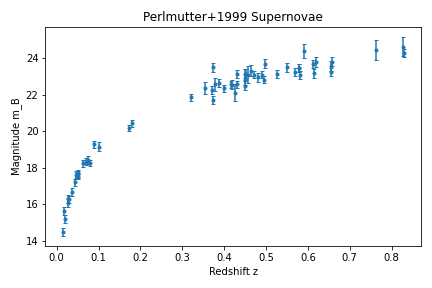
\includegraphics[height=0.45\textwidth]{pm1}}%
  \only<2>{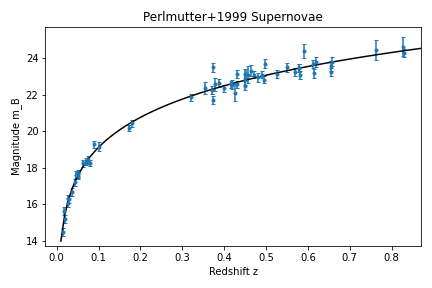
\includegraphics[height=0.45\textwidth]{pm2}}%
  \only<3>{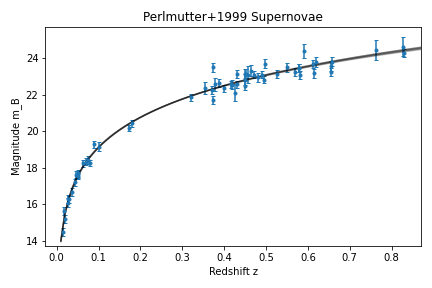
\includegraphics[height=0.45\textwidth]{pm3}}%
\end{frame}

\begin{frame}{An example}
  \begin{itemize}
    \item Then they ran MCMC...
    \item Resulting parameter constraints (blue ellipse):
  \end{itemize}
  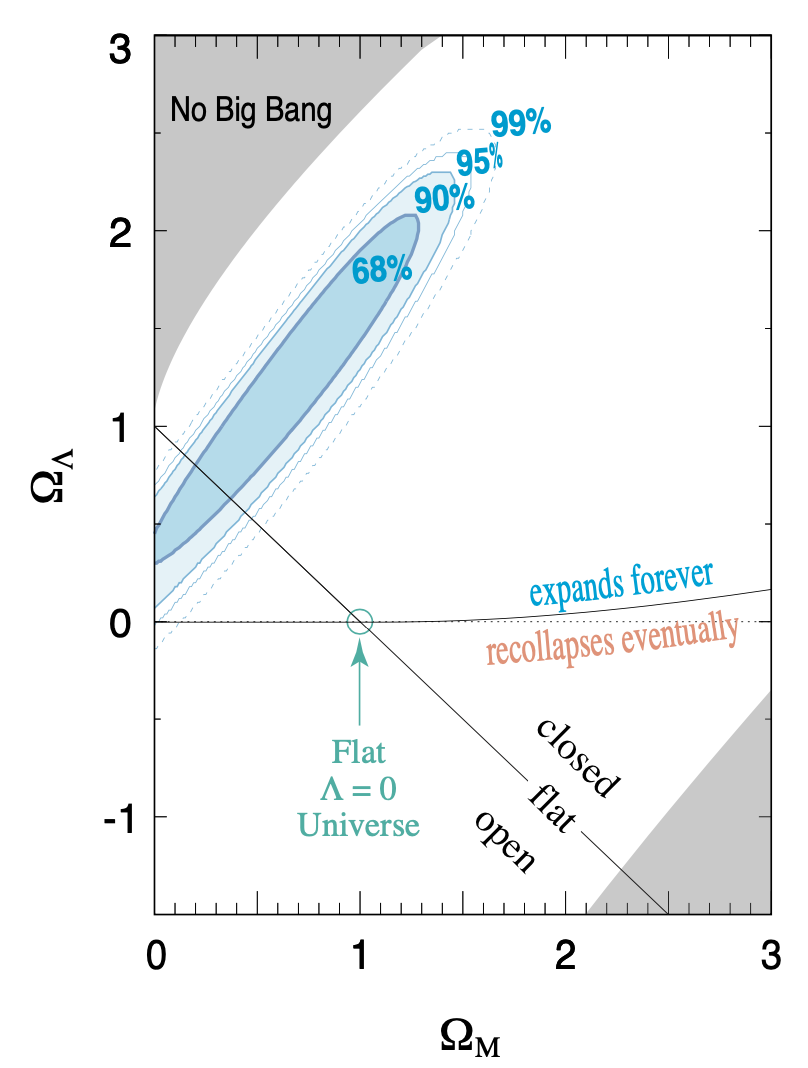
\includegraphics[height=0.6\textwidth]{pm-constraints}
\end{frame}

\begin{frame}{Why we often need MCMC}
  \begin{itemize}
  %\item We want to put \alert{constraints on the parameters} of a physical model
  %  \alert{based on observations}
  % \item constraints = posterior $= p( \textrm{parameters} | \textrm{data} )$ \\
  %   %\hspace{3em}
  %   %\small{(``The stellar mass of the Andromeda galaxy is $10 \pm 2 \times 10^{10} \textrm{M}_{\odot}$'')}
  %   \small{``The matter content of the universe (assuming flat $\Lambda$CDM) is $\Omega_{M} = 0.28 \pm 0.09$''}
  % \item $\propto \textrm{prior} \times \textrm{likelihood}$
  % \item $\propto p( \textrm{parameters} ) \times p( \textrm{data} | \textrm{parameters} )$
  % %\item We've seen examples with \alert{linear models} and \alert{Gaussian} likelihoods
  % %\item \cdots which can be solve using linear algebra
  \item Real-life models and likelihoods are often complex
  \item $\ldots$ so the resulting \alert{constraints} have complicated distributions (not Gaussians!)
    %\item We want to be able to \alert{marginalize} over ``nuisance'' parameters
  \item $\ldots$ but we can represent them with \alert{samplings}
  \item MCMC is used for drawing samples from probability distributions
        that we can compute numerically but cannot solve analytically
  \end{itemize}
\end{frame}

\begin{frame}{Samplings to represent constraints - examples}
  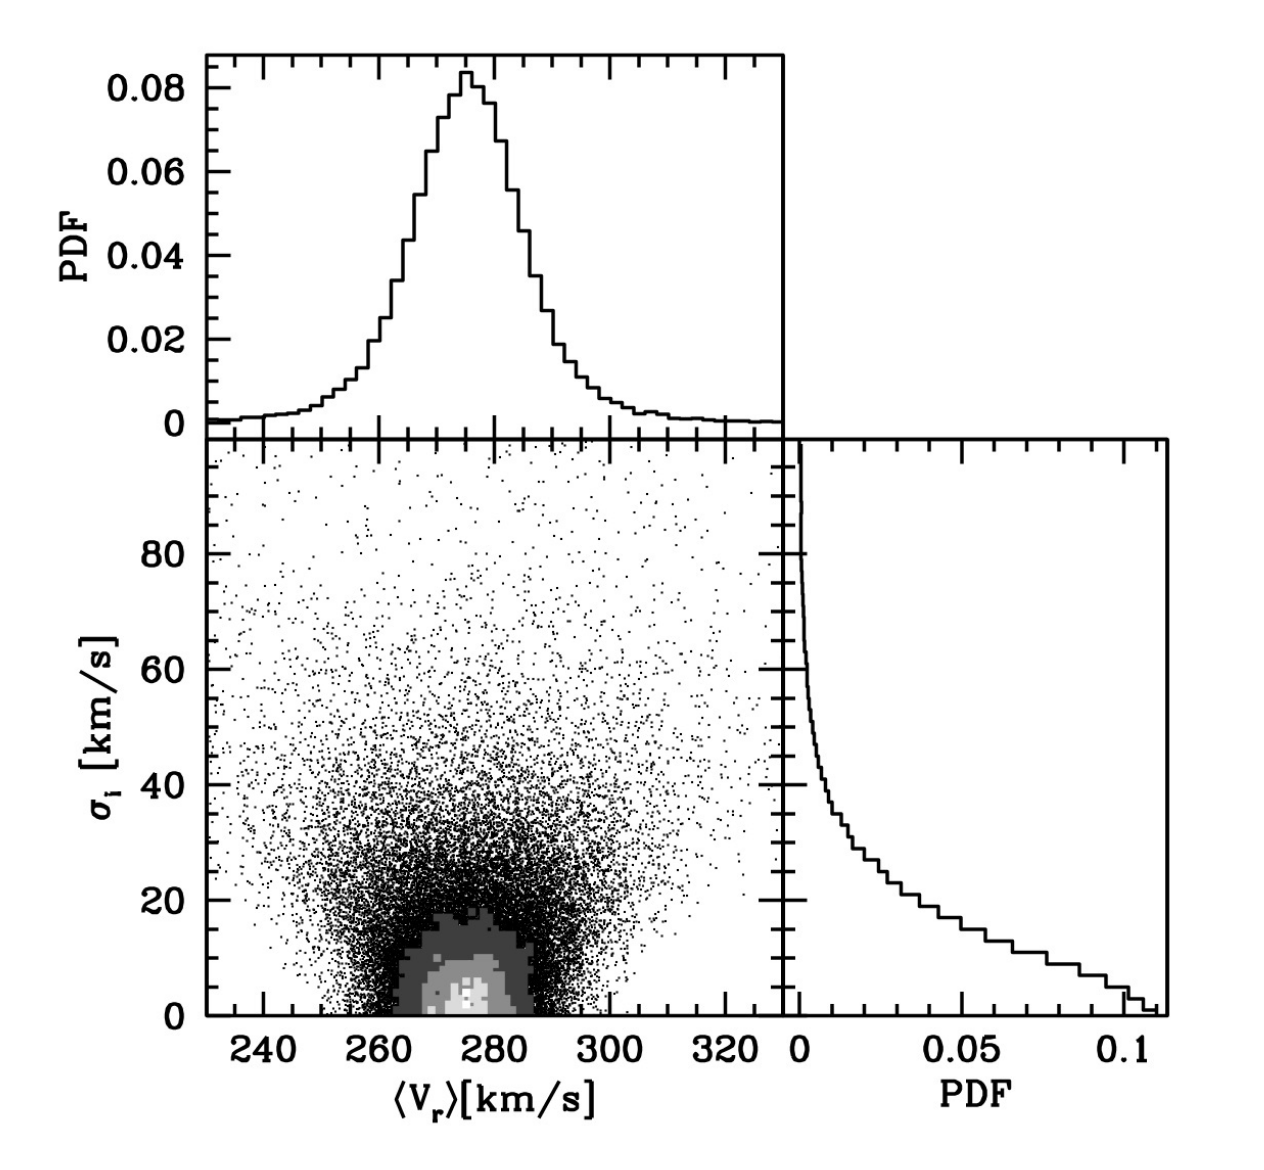
\includegraphics[height=0.5\textwidth]{corner}
  \begin{itemize}
  \item From https://arxiv.org/abs/1910.04899
  \item With a sampling: \alert{Marginalize} over a parameter by projecting it out
  \end{itemize}
\end{frame}

\begin{frame}{Samplings to represent constraints - examples}
  %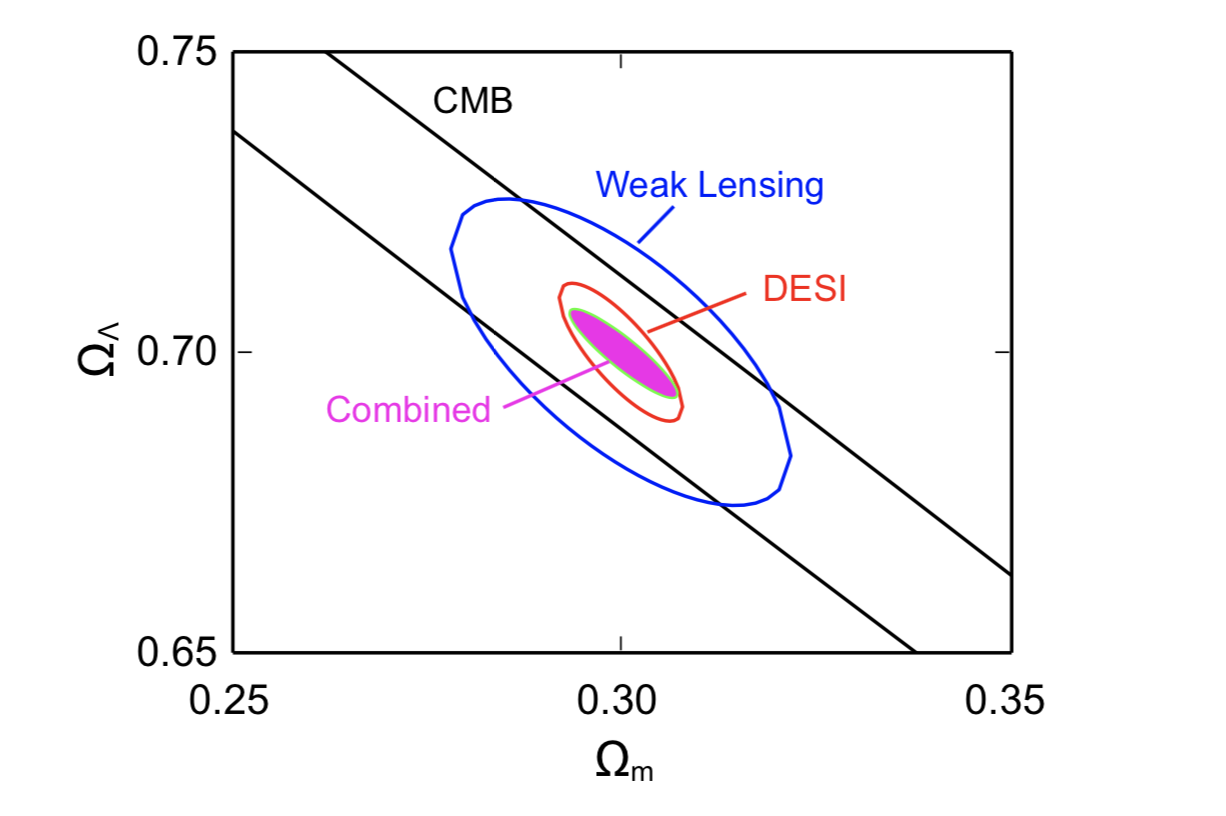
\includegraphics[height=0.5\textwidth]{banana}
  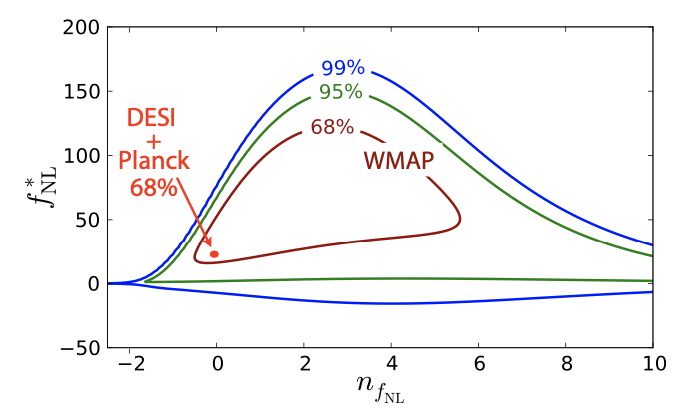
\includegraphics[height=0.5\textwidth]{fnl}
  \begin{itemize}
    \item From https://arxiv.org/abs/1611.00036
  \end{itemize}
\end{frame}

\dfmpage{30-34}

\fixequation
\dfmpage{35}

\fixequation
\dfmpage{36}

\fixequation
\dfmpage{37}

% {
% \setbeamercolor{background canvas}{bg=}
% \includepdf[pages=35,pagecommand={%
% \begin{tikzpicture}%
% (0,0) node(x) {Hello World!}
% \end{tikzpicture}}]{dfm.pdf}
% }

\dfmpage{38-39}

\fixequationx
\dfmpage{40}
\fixequationx
\dfmpage{41}

\dfmpage{42-45}

%\dfmpage{16}

% \begin{frame}{Note}
% \begin{itemize}
% \item In the previous slides, there is an unfortunate typo!  In all cases,
% \[ p(\textrm{accept}) = \min( 1, \frac{p(x)}{p(x')} \frac{q(x; x')}{q(x'; x)}) \]
% should actually be
% \[ p(\textrm{accept}) = \min( 1, \frac{p(x')}{p(x)} \frac{q(x'; x)}{q(x; x')}) \]
% That is, \alert{how good is the new place} divided by \alert{how good was the old place?}
% \end{itemize}
% \end{frame}

\begin{frame}{About the name}
\begin{itemize}
\item \alert{Monte Carlo}: a reference to the famous Monte Carlo Casino in Monaco, alluding to the randomness used in the algorithm
\item \alert{Markov Chain}: a list of samples, where each one is generated by a process that only looks at the previous one.
\item \alert{Markov}: a 19th-centure Russian mathematician and impressive-moustache-haver
with an \href{https://en.wikipedia.org/wiki/List_of_things_named_after_Andrey_Markov}{\textcolor{blue}{extensive list of things named after him}}
\item \alert{Metropolis--Hastings}: lead authors of 1953 and 1970 papers (resp.) giving the algorithm with symmetric and general proposal distributions (resp.)
\end{itemize}
\end{frame}

% \begin{frame}[containsverbatim]{The Algorithm}
% \begin{small}
% \begin{minted}{python}
% def mcmc(prob_func, propose_func, initial_pos, nsteps):
%      p = initial_pos
%      prob = prob_func(p)
%      chain = []
%      for i in range(nsteps):
%          # propose a new position in parameter space
%          p_new = propose_func(p)
%          # compute probability at new position
%          prob_new = prob_func(p_new)
%          # decide whether to jump to the new position
%          #...
%          # save the position
%          chain.append(p)
%      return chain
% \end{minted}
% \end{small}
% \end{frame}

%%%%% PYTHON %%%%%

% \begin{frame}[fragile]{The Algorithm (1)}
% \begin{small}
% \begin{minted}{python}
% def mcmc(prob_func, propose_func, initial_pos, nsteps):
%      p = initial_pos
%      prob = prob_func(p)
%      chain = []
%      for i in range(nsteps):
%          # propose a new position in parameter space
%          # ...
%          # compute probability at new position
%          # ...
%          # decide whether to jump to the new position
%          if # ...
%              # ...
%              # ...
%          # save the position
%          chain.append(p)
%      return chain
% \end{minted}
% \end{small}
% \end{frame}
% 
% \begin{frame}[fragile]{The Algorithm (2)}
% \begin{small}
% \begin{minted}{python}
% def mcmc(prob_func, propose_func, initial_pos, nsteps):
%      p = initial_pos
%      prob = prob_func(p)
%      chain = []
%      for i in range(nsteps):
%          # propose a new position in parameter space
%          p_new = propose_func(p)
%          # compute probability at new position
%          prob_new = prob_func(p_new)
%          # decide whether to jump to the new position
%          if prob_new / prob > uniform_random():
%              p = p_new
%              prob = prob_new
%          # save the position
%          chain.append(p)
%      return chain
% \end{minted}
% \end{small}
% \end{frame}
% 
% \begin{frame}[fragile]{The Algorithm (3)}
% \begin{small}
% \begin{minted}{python}
% def mcmc(logprob_func, propose_func, initial_pos, nsteps):
%      p = initial_pos
%      logprob = logprob_func(p)
%      chain = []
%      for i in range(nsteps):
%          # propose a new position in parameter space
%          p_new = propose_func(p)
%          # compute probability at new position
%          logprob_new = logprob_func(p_new)
%          # decide whether to jump to the new position
%          if exp(logprob_new - logprob) > uniform_random():
%              p = p_new
%              logprob = logprob_new
%          # save the position
%          chain.append(p)
%      return chain
% \end{minted}
% \end{small}
% \end{frame}
% 
% \begin{frame}[fragile]{The Algorithm (4)}
% \begin{small}
% \begin{minted}{python}
% def mcmc(logprob_func, propose_func, initial_pos, nsteps):
%      p = initial_pos
%      logprob = logprob_func(p)
%      chain = []
%      naccept = 0
%      for i in range(nsteps):
%          # propose a new position in parameter space
%          p_new = propose_func(p)
%          # compute probability at new position
%          logprob_new = logprob_func(p_new)
%          # decide whether to jump to the new position
%          if exp(logprob_new - logprob) > uniform_random():
%              p = p_new
%              logprob = logprob_new
%              naccept += 1
%          # save the position
%          chain.append(p)
%      return chain, naccept/nsteps
% \end{minted}
% \end{small}
% \end{frame}


\begin{frame}[fragile]{The Algorithm (1)}
\begin{footnotesize}
\begin{minted}{julia}
function mcmc(prob_func, propose_func, initial_pos, nsteps)
    p = initial_pos
    prob = prob_func(p)
    chain = []
    for i in 1:nsteps
        # propose a new position in parameter space
        # ...
        # compute probability at new position
        # ...
        # decide whether to jump to the new position
        if # ...
            # ...
            # ...
        end
        # save the position
        append!(chain, p)
    end
    return chain
end
\end{minted}
\end{footnotesize}
\end{frame}

\begin{frame}[fragile]{The Algorithm (2)}
\begin{footnotesize}
\begin{minted}{julia}
function mcmc(prob_func, propose_func, initial_pos, nsteps)
    p = initial_pos
    prob = prob_func(p)
    chain = []
    for i in 1:nsteps
        # propose a new position in parameter space
        p_new = propose_func(p)
        # compute probability at new position
        prob_new = prob_func(p_new)
        # decide whether to jump to the new position
        if prob_new / prob > uniform_random()
            p = p_new
            prob = prob_new
        end
        # save the position
        append!(chain, p)
    end
    return chain
end
\end{minted}
\end{footnotesize}
\end{frame}

\begin{frame}[fragile]{The Algorithm (3)}
\begin{footnotesize}
\begin{minted}{julia}
function mcmc(logprob_func, propose_func, initial_pos, nsteps)
    p = initial_pos
    logprob = logprob_func(p)
    chain = []
    for i in 1:nsteps
        # propose a new position in parameter space
        p_new = propose_func(p)
        # compute probability at new position
        logprob_new = logprob_func(p_new)
        # decide whether to jump to the new position
        if exp(logprob_new - logprob) > uniform_random()
            p = p_new
            logprob = logprob_new
        end
        # save the position
        append!(chain, p)
    end
    return chain
end
\end{minted}
\end{footnotesize}
\end{frame}

\begin{frame}[fragile]{The Algorithm (4)}
\begin{footnotesize}
\begin{minted}{julia}
function mcmc(logprob_func, propose_func, initial_pos, nsteps)
    p = initial_pos
    logprob = logprob_func(p)
    chain = []
    naccept = 0
    for i in 1:nsteps
        # propose a new position in parameter space
        p_new = propose_func(p)
        # compute probability at new position
        logprob_new = logprob_func(p_new)
        # decide whether to jump to the new position
        if exp(logprob_new - logprob) > uniform_random():
            p = p_new
            logprob = logprob_new
            naccept += 1
        end
        # save the position
        append!(chain, p)
    end
    return chain, naccept/nsteps
end
\end{minted}
\end{footnotesize}
\end{frame}





%
%
%


\begin{frame}{Practicalities}
\begin{itemize}
\item How do I choose a proposal distribution?
\item How many steps do I have to take?
\end{itemize}
\end{frame}

\dfmpage{46-54}

\dfmpage{59-62}

\begin{frame}{A connection to symmetries}
\begin{itemize}
\item In Metropolis--Hastings MCMC, the \emph{proposal distribution} needs
\alert{tuning parameters}, especially as dimensionality increases
\item Can be seen as a lack of \alert{symmetry} in the algorithm---the algorithm is
sensitive to the parameterization of the problem
\item For example, it's not invariant to an \alert{affine} transformation
\item \alert{Next lecture}, I'll show you an alternative algorithm that \alert{does} have affine invariance
\end{itemize}
\begin{center}
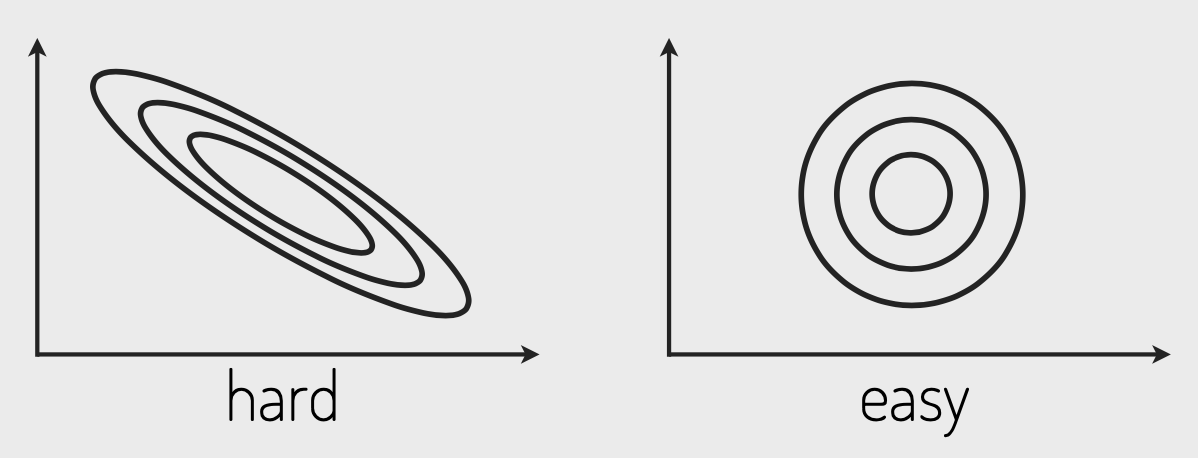
\includegraphics[width=0.6\textwidth]{hardeasy}
\end{center}
\end{frame}


\begin{frame}{How many samples do I need?}
\begin{itemize}
\item Burn-in --- skip the first $N$ samples
\item \emph{Has my chain converged?}
\item MCMC produces \alert{correlated} samples, so
  \begin{itemize}
  \item How correlated are my samples?
  \onslide<2->{
  \begin{itemize}
  \addtolength{\itemsep}{0.5ex}%
  \item Can measure the \emph{autocorrelation time} $\tau$
  \item Keep $1/\tau$ of the MCMC samples
  \item eg \niceurl{https://github.com/dfm/acor}
  \end{itemize}
  }
  \item How many uncorrelated samples do I need?
  \onslide<3->{
  \begin{itemize}
  \addtolength{\itemsep}{0.5ex}%
  \item No easy general answer to this question!
  \item ``How many can you afford?''
  \end{itemize}
  }
  \end{itemize}
\end{itemize}
\end{frame}

%\dfmpage{29}


\begin{frame}{Conclusions}
\begin{itemize}
  \addtolength{\itemsep}{0.5ex}%
\item MCMC remains an essential tool for probabilistic inference
\item For science: lets us contrain model parameters based on data (Bayesian inference)
\item Beguilingly simple algorithm, but difficult practicalities %(with some pitfalls!)
%\item A good proposal function can be hard to come up with! (and is essential for good performance!)
\item MCMC has beautiful theoretical guarantees... as compute time $\to \infty$
\end{itemize}
\end{frame}



% \begin{frame}{This afternoon's tutorial/lab session}
% \begin{itemize}
% \item Bob Room, 3:15--4:30
% \item Time to play with MCMC yourself!
% \item We'll use Google CoLab - no need to install anything on your computer
% \item In the Python language
% \end{itemize}
% \end{frame}




\end{document}

